\section{Summary}
This dissertation has demonstrated that it is possible to develop collaborative, multi-platform AR solutions for education thanks to a modular architecture that provides useful functionalities for both software developers and educators. This work has been possible thanks to an extensive collaboration between researchers, educators and software developers, as well as through the participation in the ARETE project. 

At first, an extensive study of the state-of-the-art was performed to analyse recent research work where AR applications for education were described. The aim of the study was threefold:
\begin{itemize}
    \item Identify the works describing interactive, multi-user or collaborative AR experiences and compare their main features;
    \item Understand the motivation behind the usage of AR as an educational tool;
    \item Measure the impact of using AR in the classroom, by analysing pre-/post- test results or comparing grades versus a control group.
\end{itemize}

The systematic study of the literature clearly identified a lack of works where multi-user collaborative apps are presented, as well as the lack of a common framework providing multiplatform support for such applications. This led to the decision of developing \ork{}, an open-source library that enables real-time communication between different devices and that, thanks to C\# and Python bindings, can be used on many different platforms such as web apps, iOS or Android devices and \glspl{hmd} like the Microsoft HoloLens.

Then a collaboration with teachers from secondary schools was established to pinpoint what are the limiting factors in the adoption of AR applications in education and what these apps should provide in order to be used effectively. Based on the teachers answers, eleven requirements (summarised in Table \ref{arch:tab:summaryreqs}) were identified, and an architecture was defined based on six design objectives:
\begin{enumerate}[start=1,label={\bfseries DO\arabic*:}]
    \item Interoperability;
    \item Multi-user support;
    \item Data collection;
    \item Data visualization;
    \item AI-based analytics;
    \item Ease of development.
\end{enumerate}

An architecture named \arch{}, that fulfills all the aforementioned design objectives, was developed and tested through the development of three \glspl{poc} (\textit{ARCube}, \textit{xAPI Data Analysis} and \textit{AR Geography Quiz}). The architecture is composed of 4 different modules (Real-time multi-user interactions, Data storage, AI-based analytics and Visualisation tools). A modular architecture offers several advantages, since it allows developers to choose which parts of it should be integrated in their existing applications and it is also easier to extend and maintain.

Finally, the architecture was validated by implementing a multi-user Geography quiz. The application, called \appname{}, has been tested by 44 students with ages ranging from 13 to 19 under the supervision of 3 teachers. Through a set of post-study interviews with the teachers, the analysis of the surveys filled by the students after using the apps and the analysis of the data collected during the app usage, it was possible to demonstrate that applications based on the \arch{} architecture fulfills the requirements identified by the teachers. All the code developed during this research has been released as open-source to enable researchers to build upon this work and further enable the usage of AR solutions in the education sector.

In summary, this research provides progress beyond the state of the art for the usage of collaborative AR solutions for education, by presenting an architecture that takes into account the teachers requirements for using AR solutions at school and that can be adapted to their specific needs and integrate with the LMS of the school and provide them with valuable data to analyze the progress of the students.

\section{Contributions}\label{sec:contribs}
The main contribution of this research has been the definition of an architecture for the creation of multi-user \gls{ar} experiences across different platforms, general enough to be easily adapted to many different use cases and scenarios and ready for any technological update such as the release of new hardware devices or software libraries. 

As a result of the objectives mentioned in Section \ref{sec:objectives}, the main contribution can be translated into four specific outcomes:
\begin{enumerate}[start=1,,ref=C.\arabic*,label={\bfseries C\arabic*:}]
    \item An in-depth analysis of the state-of-the-art that allows to identify the state of current research on AR in terms of what kind of solutions are currently used in schools, what is the motivation for using AR in education and what effect does AR applications have on students motivation and retention of the topics studied. This is described in Chapter \ref{chap:sota} and reflected in publications \ref{pub:intro} and \ref{pub:sota}; \label{con:sota}
    \item The development of a multiplatform software library, called \textit{\ork{}}, which allows multi-user interactions in real-time applications. This is described in detail in Section \ref{sec:architecture:multiuser} and reflected in publication \ref{pub:ork};\label{con:ork}
    \item The definition of \arch, a modular architecture for the creation of AR solutions that satisfies all the requirements identified by teachers and that enables in a seamless fashion multi-user capabilities. This is described in Chapter \ref{chap:arch} and reflected in publications \ref{pub:beh} and \ref{pub:arch};\label{con:arch}
    \item The implementation and validation of \appname{}, an AR application based on the architecture, that has been tested in three different educational institutions and that validates all the required design objectives. This is described in Chapter \ref{chap:eval} and reflected in publications \ref{pub:eval} and \ref{pub:eval2}.\label{con:eval}
\end{enumerate}

The contributions delivered the following publications:
\begin{enumerate}[start=1,,ref=P\arabic*,label={\bfseries P\arabic*:}]
    \item Masneri, S., Domínguez, A., Wild, F., Pronk, J., Heintz, M., Tiede, J., Nistor, A., Chiazzese, G., \& Mangina, E. (2020). \textbf{Work-in-progress-ARETE-An Interactive Educational System using Augmented Reality.} In D. Economou, A. Klippel, H. Dodds, A. Pena-Rios, M. J. W. Lee, D. Beck, J. Pirker, A. Dengel, T. M. Peres, \& J. Richter (Eds.), 2020 6th International Conference of the Immersive Learning Research Network (iLRN): Conference Proceedings (pp. 283-286). \url{https://doi.org/10.23919/iLRN47897.2020.9155186} \label{pub:intro}
    \item Masneri, S., Domínguez, A., Zorrilla, M., Larrañaga, M., \& Arruarte, A. (2022). \textbf{Interactive, collaborative and multi-user augmented reality applications in primary and secondary education. A systematic review.} JUCS-Journal of Universal Computer Science, 28(6), 564-590. \url{https://doi.org/10.3897/jucs.76535} \label{pub:sota}
    \item Masneri, S., Domínguez, A., Sanz, M., Tamayo, I., Zorrilla, M., Larrañaga, M., \& Arruarte, A. (2022). \textbf{Collaborative Multi-user Augmented Reality Solutions in the Classroom.} In: Auer, M.E., Hortsch, H., Michler, O., Köhler, T. (eds) Mobility for Smart Cities and Regional Development - Challenges for Higher Education. ICL 2021. Lecture Notes in Networks and Systems, vol 390. Springer, Cham. \url{https://doi.org/10.1007/978-3-030-93907-6\_106} \label{pub:ork}
    \item Domínguez, A., Cabrero, Á., Simões, B., Chiazzese, G., Farella, M., Arrigo, M., Seta, L., Chifari, A., Tosto, C., Goei, S.L., Mangina, E. \& Masneri, S. (2023). \textbf{Collaborative Augmented Reality Tools for Behavioral Lessons.} In 25th International Conference on Interactive Collaborative Learning, ICL 2022 (pp. 102-109). Springer Science and Business Media Deutschland GmbH. \url{https://doi.org/10.1007/978-3-031-26876-2_10} \label{pub:beh}
    \item Masneri, S., Domínguez, A., Sanz, M., Zorrilla, M., Larrañaga, M., \& Arruarte, A. (2023). \textbf{cleAR: an interoperable architecture for multi-user AR-based school curricula.}  Virtual Reality 27, 1813–1825 (2023). \url{https://doi.org/10.1007/s10055-023-00764-5} \label{pub:arch}
    \item Masneri, S., Domínguez, A., Pacho, G., Zorrilla, M., Larrañaga, M., \& Arruarte, A. \textit{(Submitted in 2023, July).} \textbf{A Collaborative AR Application for Education: from Architecture Design to User Evaluation.} \label{pub:eval}
    \item Domínguez, A., Pacho, G., Bowers, L., Wild, F., Alcock, S., Chiazzese, G., Farella, M., Arrigo, M., Ross, D., Treacy, T., Yegorina, D., Mangina, E. \& Masneri, S. (2023). \textbf{Dataset of user interactions across four large pilots on the use of augmented reality in learning experiences.} Sci Data 10, 823 (2023). \url{https://doi.org/10.1038/s41597-023-02743-6} \label{pub:eval2}
\end{enumerate}

\begin{figure*}[htbp]
    \centering
    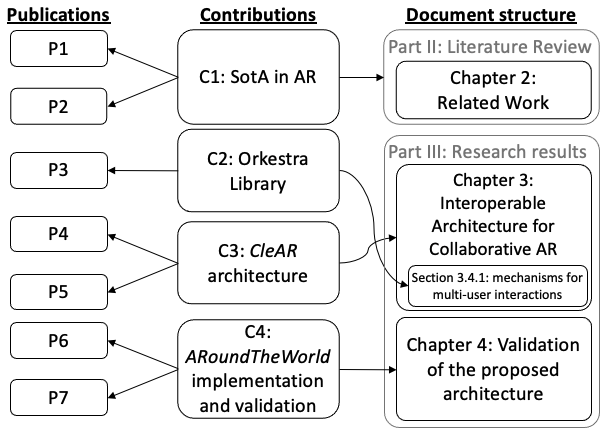
\includegraphics[width=0.95\textwidth]{Conclusions/figures/contrib_diagram.png}
    \caption{\fontsize{10pt}{11pt}\selectfont{\itshape{The relations between the work described in this document, its main contributions and the publications produced.}}}
    \label{fig:contribs}
\end{figure*}

Figure \ref{fig:contribs} summarises the contributions of this work and its related publications.
Furthermore, all the code developed is available as open source in several GitHUb repositories:

\begin{itemize}
    \item The data analysis conducted while performing the systematic literature review described in Chapter \ref{chap:sota} is available at \url{https://github.com/Stocastico/AR_SLR_Paper};
    \item \ork{} has separated repositories for the client (\url{https://github.com/tv-vicomtech/orkestraClient}) and server (\url{https://github.com/tv-vicomtech/orkestraServer}) implementations, as well as a separate one for the Unity version (\url{https://github.com/tv-vicomtech/orkestralibUnity});
    \item The 3 PoCs created for the conceptual evaluation of \arch{}, together with the (anonymised) data collected from the teachers surveys, are available at \url{https://github.com/Stocastico/ARchitecture_paper}, and the library used to simplify the analysis of xAPI statements is available at \url{https://github.com/Stocastico/xapi_analysis};
    \item The code of \appname{} is hosted at \url{https://github.com/tv-vicomtech/ARoundtheworld}, while the data collected from the students questionnaires and their analysis is available at \url{https://github.com/Stocastico/Evaluation_paper}.
\end{itemize}

\section{Future work}
Throughout the development of the research work, the analysis of the literature, the definition and evaluation of the architecture and the interviews with the teachers, several opportunities were identified to complement and extend the research presented in this work.

Developing an authoring tool which simplifies and speeds up the creation of collaborative AR experiences would enable creators to greatly increase the availability of AR educational software. While this is not a new idea \citep{rajaram2022paper, thanyadit2022easy}, so far no such software has been used to create commercial applications, and there are no authoring tools which allow incorporating collaborative capabilities in AR applications.

Related to the development of an authoring tool is the addition of AI-based tools that enable the creation of 3D models, either from static 2D images \citep{mildenhall2021nerf} or from text description \citep{poole2022dreamfusion, deitke2023objaversexl}, since the creation of the 3D assets is one of the most time-consuming tasks when developing AR content. Including such functionality in an easy-to-use way, ideally through a front-end which directly interact with the authoring tool, would enable the creation of AR apps without the need of professional software developers or 3D designers.

AI models could also be further integrated in the architecture. While a basic support is already available, both for the optimisation of parameters in the application and for supporting the analysis of the data, more advanced models such as chatGPT Code Interpreter \citep{openai2023gpt4} could fully automate the data analysis tasks, which the teachers consider hard to complete on their own. Furthermore, other generative models could be used to speed-up the development or the creation of new content.

Another future research direction revolves around enabling the \arch{} architecture to support newer hardware platforms, for example the recently released Apple AR Vision Pro. So far, the architecture supports several platforms (Microsoft HoloLens, web, Android and iOS devices), but it lacks software that enables to easily add support to other ones. Restructuring the code in such a way would make the architecture able to support a wider variety of platforms as well as making it easier to maintain in the future. 

Finally, it would be interesting to extend the scope of this research to other domains. On one side, it should be straightforward to extend the architecture to VR applications since every functionality should work out of the box, provided that support for different hardware (like Oculus Quest, for example) is added. On the other side, it would be interesting to investigate how \arch{} should be modified to support use cases in other domains such as medicine or manufacturing. Collaborative AR has several applications in these domains, but the requirements of an architecture analog to the one presented in this work are probably different from the ones described in Chapter \ref{chap:arch}, and this will in turn lead to different design objectives.

